% !TeX spellcheck = en_US

%!TEX root = ../thesis.tex
%*******************************************************************************
%****************************** Second Chapter *********************************
%*******************************************************************************


\chapter{Statistical inference}

\pagebreak

\section{Bayesian Inference}
\subsection{Định lý Bayes}
Định lý Bayes là một định lý cơ bản thường xuyên được sử dụng trong lý thuyết học máy.

\begin{equation}
	P(A/B) = \frac{P(B/A)P(A)}{P(B)}
\end{equation}
Trong đó: 
A và B là các sự kiện.

$P(A), P(B)$ : Xác suất của sự kiện A, B xảy ra tương ứng.

$P(A/B)$ là xác suất sự kiện A xảy ra nếu biết sự kiện B đã xảy ra

$P(B/A)$ là xác suất sự kiện B xảy ra nếu biết sự kiện A đã xảy ra

Định lý Bayes cho phép chúng ta sử dụng những kiến thức hay niềm tin đã có để tính toán xác suất cho một sự kiện nào đó.
\subsection{Suy luận Bayesian}
Suy luận Bayes là một phương pháp suy luận thống kê mà định lý Bayes được sử dụng để cập nhật xác suất của một giả thuyết khi có thêm nhiều thông tin hay bằng chứng hơn. 

Một phần quan trọng của suy luận Bayes là việc thiết lập các tham số và mô hình. Mô hình là một công thức toán học của bộ dữ liệu quan sát được. Tham số là các yếu tố trong mô hình ảnh hưởng đến dữ liệu.
Để xây dựng một mô hình, ta cần thiết kế cấu trúc và ước lượng bộ tham số của nó.
Giá sử $\Theta$ đại diện cho bộ tham số của mô hình, $y = \{y_1, y_2, \dots, y_n \}$ là bộ dữ liệu mà chúng ta có được. Lúc này, định lý Bayes được viết dưới dạng:
\begin{equation}
P(\Theta/y) = \frac{P(y/\Theta)P(\Theta)}{P(y)}
\end{equation}
$P(y/\Theta)$ được gọi là \textit{Likelihood}, mô tả tính hợp lý của giá trị tham số mô hình từ các dữ liệu quan sát được.

$P(\Theta)$ được gọi là phân phối tiền nghiệm hay \textit{prior}, đại diện cho những kiến thức, niềm tin về giá trị thực của tham số từ những kinh nghiệm trước đây khi chưa tiếp xúc với dữ liệu hiện tại.

$P(\Theta/y)$ được gọi là phân phối hậu nghiệm hay \textit{posterior}. Nó đại diện cho phân phối của các tham số sau khi đã quan sát được bộ dữ liệu \textit{y}.

$P(y)$ được gọi là phân phối cận biên hay chứng cứ, nó giúp chuẩn hóa đầu ra của \textit{posterior}, đảm bảo \textit{posterior} thõa điều kiện là một phân phối xác suất.

Trong một vài trường hợp, chúng ta không quan tâm đến việc liệu phân phối có được chuẩn hóa hay không. Khí đó, chúng ta có thể viết lại định lý Bayes dưới dạng rút gọn hơn:
\begin{equation}
P(\Theta/y) \propto P(y/\Theta)P(\Theta)
\end{equation}
\textit{Một số lưu lý về prior}
\textit{Prior} là một sự đặc biệt trong suy luận Bayes, giúp đưa những kiến thức đã biết hay kiến thức của chuyên gia về $\Theta$ vào việc hình thành nên mô hình, làm cho mô hình thu được không phụ thuộc hoàn toàn dữ liệu, ngăn chặn được tình trạng \textit{overfitting} khi có ít dữ liệu.

\textit{Prior} có nhiệm vụ bảo vệ (một phần nào đó) kiến thức đã có về mô hình khỏi những dữ liệu nhiễu. \textit{Prior} có sức ảnh hưởng mạnh nhất khi mô hình chưa được học với quá nhiều dữ liệu.
\begin{figure}[h]
	\begin{center}
		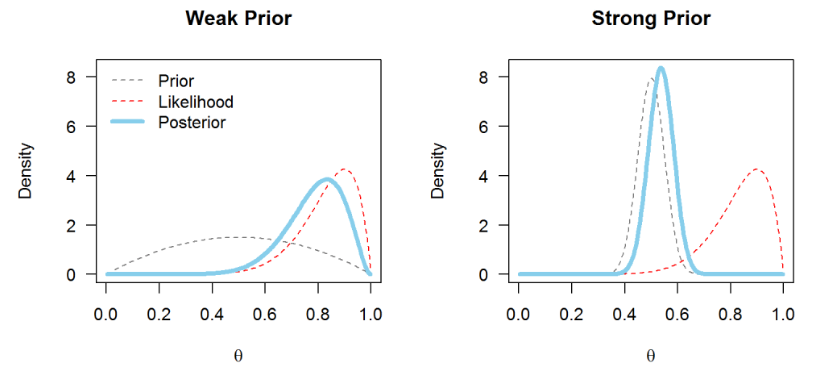
\includegraphics[height=.25\textheight]{Chuong3/Figs/prior.png}
		\label{fig:su anh huong cua prior}
		\caption{Sự ảnh hưởng của một \textit{prior} yếu và một \textit{prior} mạnh khi tung đồng xu được 9/10 mặt ngửa}
	\end{center}
\end{figure}
Trong thực thế, đặc biệt là trong việc đào tạo mô hình, việc nhận định sai về $\Theta$ hay Prior sai rất dễ xảy ra. Trong trường hợp này, chỉ cần thu thập thật nhiều dữ liệu. Khi ấy, sự ảnh hưởng của Prior ngày càng giảm dần, Posterior vẫn sẽ hội tụ đến đến điểm tối ưu. Điều này được minh họa ở hình \ref{fig:su anh huong cua prior sai}
\begin{figure}[h]
	\begin{subfigure}{.5\textwidth}
	\centering
	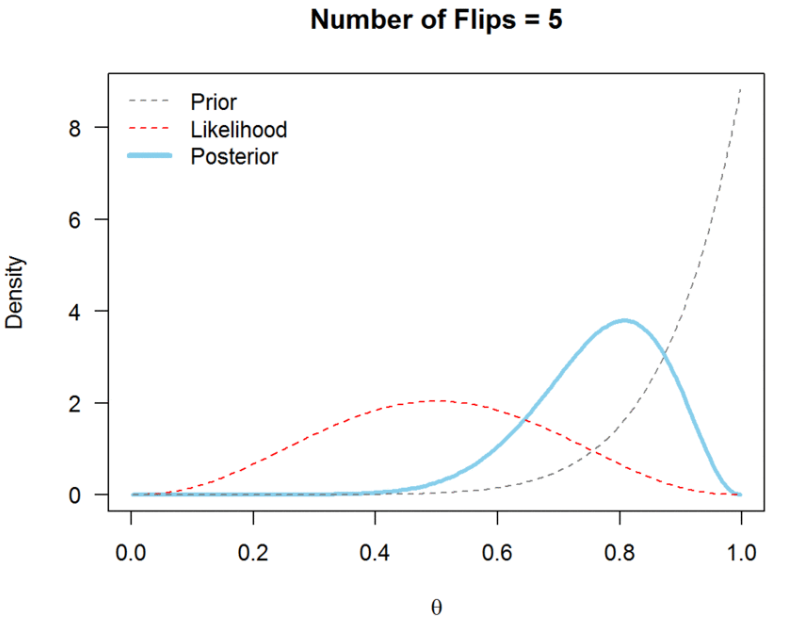
\includegraphics[width=.8\linewidth]{Chuong3/Figs/5.png}
	\label{fig:sfig1}
	\end{subfigure}
	\begin{subfigure}{.5\textwidth}
	\centering
	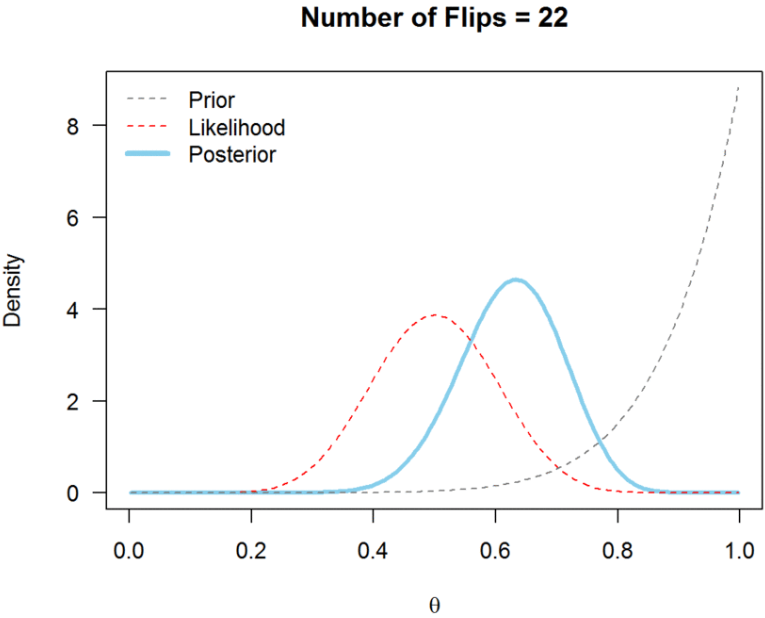
\includegraphics[width=.8\linewidth]{Chuong3/Figs/22.png}
	\label{fig:sfig1}
	\end{subfigure}
	\begin{subfigure}{.5\textwidth}
	\centering
	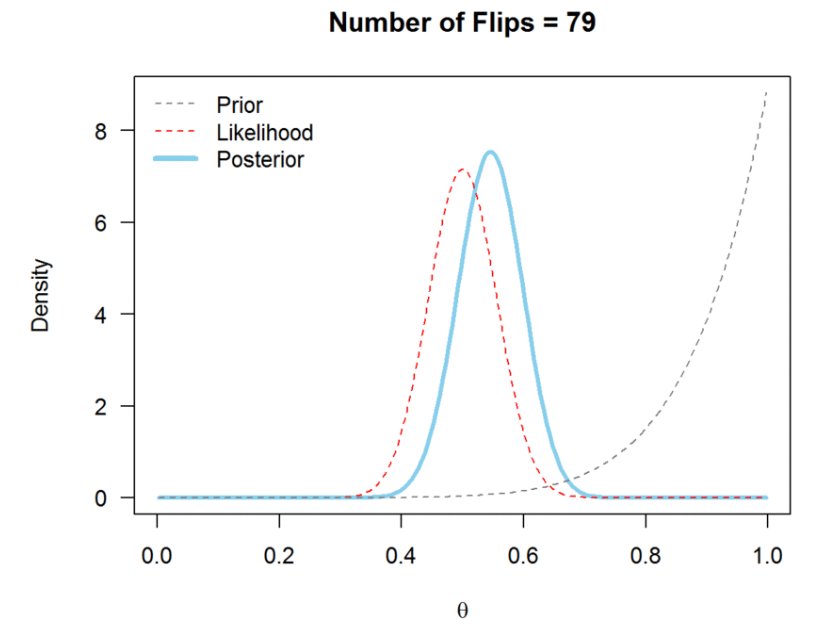
\includegraphics[width=.8\linewidth]{Chuong3/Figs/79.png}
	\label{fig:sfig1}
	\end{subfigure}
	\begin{subfigure}{.5\textwidth}
	\centering
	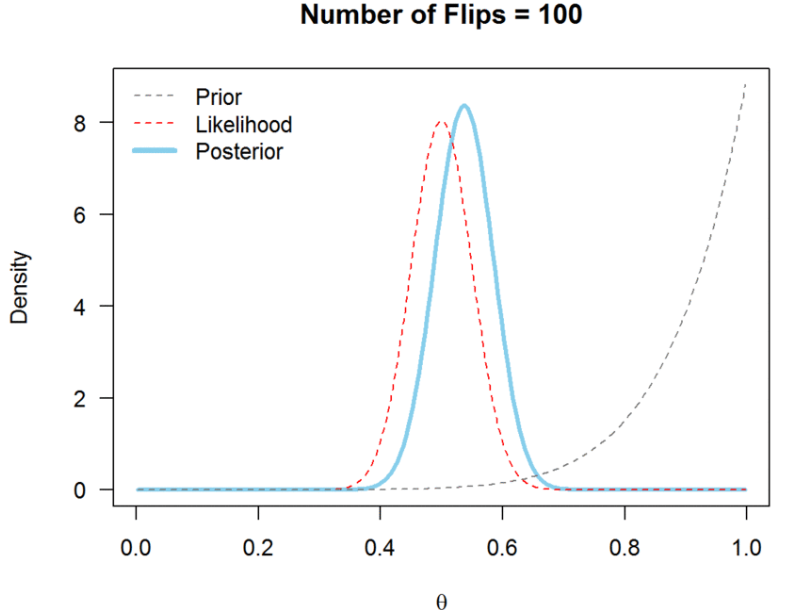
\includegraphics[width=.8\linewidth]{Chuong3/Figs/100.png}
	\label{fig:sfig1}
	\end{subfigure}
	\label{fig:su anh huong cua prior sai}
	\caption{Cùng với một prior khá lệch, khi ta tung đồng xu càng nhiều thì posterior càng hội tụ đến LikeLihood}
\end{figure}


\section{Variational Inference}
\subsection{Probabilistic model}
Một mạng thần kinh có thể được xem như mộng mô hình xác suất $p(y/x,w)$. Trong nhiệm vụ phân loại, $y$ là tập hợp các phân lớp và  $p(y/x,w)$ là một phân phối phân loại. Trong nhiệm vụ hồi quy, $y$ là một biến liên tục và  $p(y/x,w)$ là một phân phối Gaussian.

Cho tập dữ liệu đào tạo $\mathcal{D}={\textbf{x}^{(i)},y^{(i)}}$, chúng ta có thể xây dựng Likelihood $p(\mathcal{D}/\textbf{w}) = \prod_{i}p(y^{(i)}|\textbf{x}^{(i)},\textbf{w})$ là một hàm số của $\textbf{w}$. Cực đại hóa Likelihood (MLE) cũng là một phương pháp hay dùng để tìm $\textbf{w}$ tối ưu nhưng nó dễ dẫn đến onverfiting vì phụ thuộc hoàn toàn vào dữ liệu.

Nhân Likelihood với một Prior $p(\textbf{w})$ sẽ tỷ lệ với phân phối Posterior $p(\textbf{w}/\mathcal{D}) \propto p(\mathcal(D/\textbf{w})p(\textbf{w}))$. Cực đại hóa $p(\mathcal(D/\textbf{w})p(\textbf{w}))$ tương đương bởi tìm $\textbf{w}$ để Posterior $p(\textbf{w}/\mathcal{D})$ đạt giá trị lớn nhất (hay được gọi là MAP). Làm việc với MAP cho hiệu quả tổng quát hơn và có thể ngăn chặn overfitting.

MLE và MAP đều ước lượng điểm cho các tham số trong mô hình. Thay vào đó, nếu chúng ta có phân phối Posterior đầy đủ cho tất cả các tham số, chúng ta có thể đưa ra nhiều dự đoán với những tham số được lấy ngẫu nhiên từ Posterior. Khi ấy, không những ta thu được dự đoán có tính tổng quát cao mà còn đánh giá được độ không chắc chắn của dự đoán ấy. Khi đó, mục tiêu tối ưu hóa hay hàm mất mát được viết dưới dạng
\begin{equation*}
p(y/\textbf{x},\mathcal{D}) = \int p(y/\textbf{x},\textbf{w})p(\textbf{w}/\mathcal{D})d\textbf{w}
\end{equation*}
Điều này tương đương với trung bình các dự đoán đến từ các mạng thần kinh có trong số được lấy từ phân phối Posterior.
\subsection{Variational Inference}
Thật không may, việc ước lượng Posterior $p(y/\textbf{x},\mathcal{D})$ trong mạng thần kinh rất khó khăn vì trong đó, số lượng tham số rất lớn, có thể đến hàng triệu tham số. Vì thế, chúng ta phải ước lượng Posterior bằng một phân phối $p(\textbf{w}/\theta)$ có dạng đơn giản hơn. Việc cực tiểu hóa KL divergence giữa $p(\textbf{w}/\theta)$ và phân phối Posterior $p(y/\textbf{x},\mathcal{D})$ có thể giúp ta làm việc này. Nhiệm vụ của ta là tìm điểm tối ưu $\theta^*$ của $\theta$ để KL divergence đạt cực tiểu.
\begin{align*}
\theta^* &= \arg\min_{\theta}\textbf{KL}[q(\textbf{w}|\theta)||P(\textbf{w}|\mathcal{D})] \\
& = \arg\min_{\theta}\displaystyle \int q(\textbf{w}|\theta)log\frac{q(\textbf{w}|\theta)P(\mathcal{D})}{P(\textbf{w})P(\mathcal{D}|\textbf{w})}d\textbf{w} \\
& = \arg\min_{\theta}\displaystyle \int q(\textbf{w}|\theta)(log\frac{q(\textbf{w}|\theta)}{P(\textbf{w})}-log(P(\mathcal{D}|\textbf{w}))+ log(P(\mathcal{D})))d\textbf{w} \\
& = \arg\min_{\theta}\textbf{KL}[q(\textbf{w}|\theta)||P(\textbf{w})] - \mathbb{E}_{q(\textbf{w}|\theta)}[\log P(\mathcal{D}|\textbf{w})] + \mathbb{E}_{q(\textbf{w}|\theta)}[\log P(\mathcal{D})] \\
& = \arg\min_{\theta}\textbf{KL}[q(\textbf{w}|\theta)||P(\textbf{w})] - \mathbb{E}_{q(\textbf{w}|\theta)}[\log P(\mathcal{D}|\textbf{w})] \\
\end{align*}
$\log P(\mathcal{D})$ có thể được bỏ qua trong việc tối ưu hóa vì nó là hằng số.
Để đơn giản, ta có thể định nghĩa hàm mất mát:
\begin{align*}
\mathcal{F}(\mathcal{D},\theta) &= \textbf{KL}[q(\textbf{w}|\theta)||p(\textbf{w})] - \mathbb{E}_{q(\textbf{w}|\theta)}[\log P(\mathcal{D}|\textbf{w})]  \\
& = \mathbb{E}_{q(\textbf{w}|\theta)}\log p(w|\theta) - \mathbb{E}_{q(\textbf{w}|\theta)}\log p(w) - \mathbb{E}_{q(\textbf{w}|\theta)}\log p(\mathcal{D}|\textbf{w}) \\
& \approx\frac{1}{N}\sum_{i = 1}^{N}[\log p(w^{(i)}|\theta) - \log p(w^{(i)}) - \log p(\mathcal{D}|w^{(i)})]\\
\end{align*}
\section{Uncertainties in Bayesian Learning}

Sự không chắc chắn của một mạng thần kinh là độ đo thể hiện sự chắc chắn bao nhiêu của mô hình với dự đoán của nó. Trong mô hình Bayesian, có 2 loại không chắc chắn chính: Aleatoric và Epistemic.
Độ không chắc chắn Aleatoric đo tính không chắc chắn có của dữ liệu. Ví dụ, trong các vấn đề với ảnh, các vị trí mà đối tượng bị che khuất hoặc thiếu các đặc điểm nhận dạng thưởng có đô không chắn chắn Aleatoric cao.


Độ không chắc chắn Epistemic thể hiện sự thiếu thông tin về dữ liệu của mô hình. Epistemic cao với những trường hợp mà mô hình chưa được học và ta có thể giảm nó nếu cung cấp đủ dữ liệu.

\begin{figure}[h]
	\begin{center}
		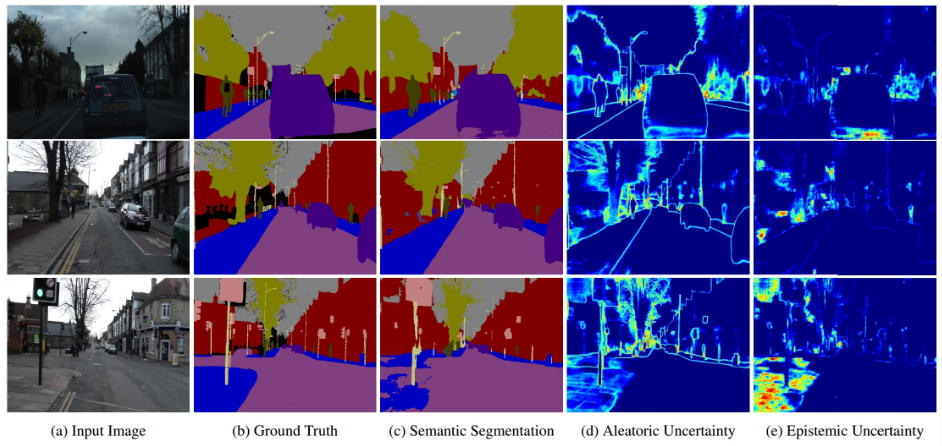
\includegraphics[height=.25\textheight]{Chuong3/Figs/uncertainty.png}
		\label{fig:minh hoa uncertainty}
		\caption{Một ví dụ của uncertainty trong bài toán Semamtation}
	\end{center}
\end{figure}



